\documentclass[withoutpreface,bwprint]{cumcmthesis}

\title{基于SEIR改进模型的疫情应对措施分析}

\begin{document}
\maketitle

\section{项目背景}
人类社会面临传染病的严重威胁,近几年发生的一些传染病,如非典型性肺炎(SARS)、
高致病性禽流感H5N1,甲型流感H1N1,新型冠状病毒肺炎(COVID-19)等,均对生命健康
和社会生活造成了很大的影响,如何遏制传染病爆发、缓解传染病流行,是当今社会面临的
紧迫问题,从系统科学的角度看,传染病流行时在人群中发生的一个复杂扩散过程,对这一过程进行
建模,有助于理解传染病的流行机理,认识内在规律,为干预措施的选择提供理论依据。

\section{研究内容}
\subsection{模型选择}
目前,对传染病流行过程的建模已经发展出了多种范式,概括来说,可以分为:单一群体方法、
复合群体方法和微观个体方法。主要有三种方法 第一种是单一群体方法:将人群看作一个整,流
行过程表现在易感者,感染者等各类人员集计量的变化;第二种是复合群体方法:考虑人群在空间上的异质
性,将人群划分为多个子群体,各子群体之间因人员流动而藕合,形成复杂动态系统;第三种
是微观个体方法:建模出发点是人群中的个体,个体有各自的属性和行为规则,个体之间形成接触网络,感染
者和易感者的接触导致易感个体状态的变化,形成网络上的传播动力学过程。三种建模方法的基本思想如\cref{fig:1}。
\begin{figure}[!h]
    \centering
    \begin{minipage}[c]{0.3\textwidth}
        \centering
        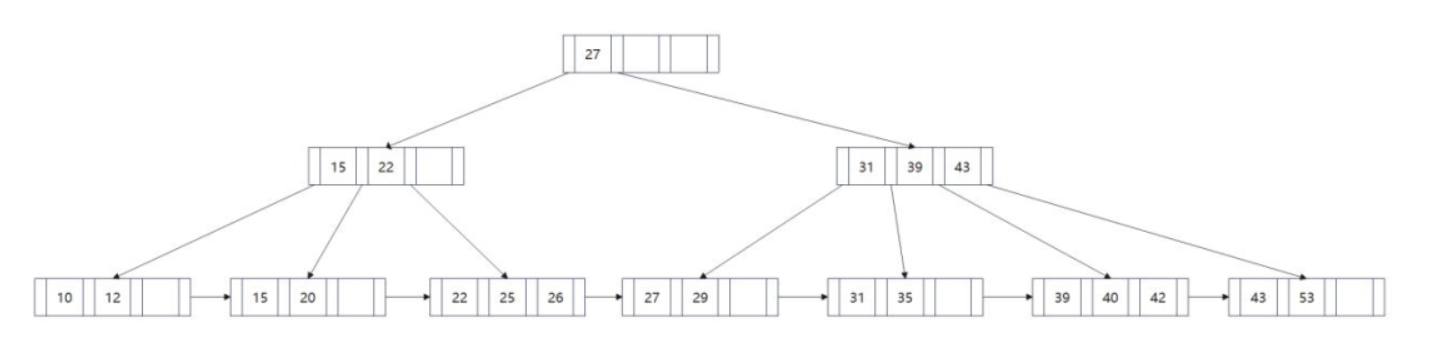
\includegraphics[width=0.95\textwidth]{2}
        \subcaption{单一群体方法}
        \label{fig:1.1}
    \end{minipage}
    \begin{minipage}[c]{0.3\textwidth}
        \centering
        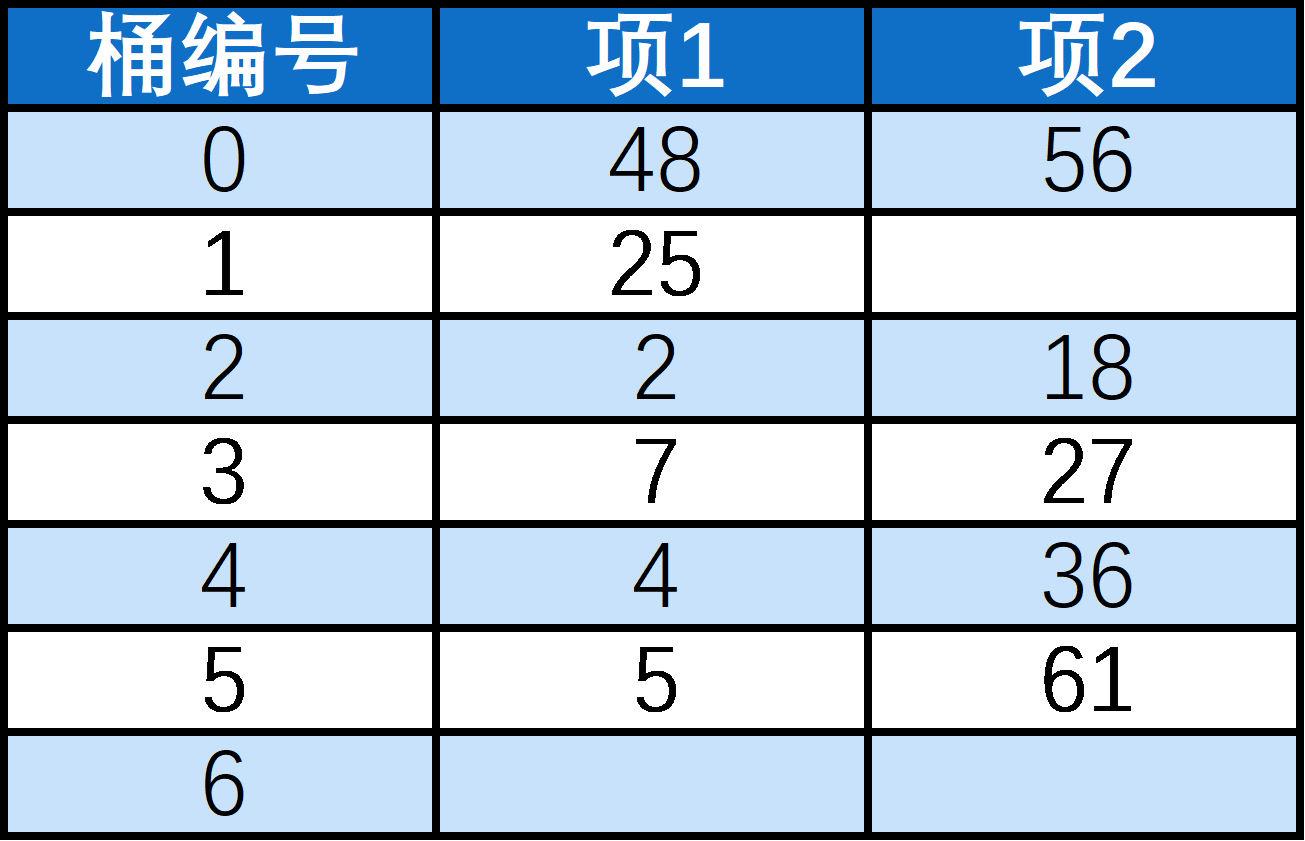
\includegraphics[width=0.95\textwidth]{3}
        \subcaption{复合群体方法}
        \label{fig:1.2}
    \end{minipage}
    \begin{minipage}[c]{0.3\textwidth}
        \centering
        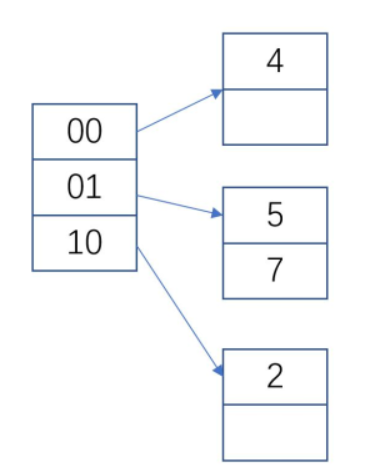
\includegraphics[width=0.95\textwidth]{1}
        \subcaption{微观个体方法}
        \label{fig:1.3}
    \end{minipage}
    \caption{传染病传播三种建模方法}
    \label{fig:1}
\end{figure}

\par
在这里,选择单一群体方法中的SEIR模型作为基础模型,如\cref{fig:2},在基于SEIR模型的改进模型上进行分析。
\begin{figure}[!h]
    \centering
    \includegraphics[width=0.95\textwidth]{SEIR_model}
    \caption{SEIR模型}
    \label{fig:2}
\end{figure}

\subsection{模型改进}
\subsubsection{模型拓扑结构的改进}
传统的SEIR模型将人群分为易感人群、潜伏期人群、感染人群和康复人群。人群划分较为粗糙,
与现实情况拟合结果较差。

而在应对2019年底开始的新型冠状病毒肺炎疫情中,隔离措施被实践证明是一种有效的减缓传染病流行的措施。
将隔离措施纳入考虑,进一步将易感人群、潜伏期人群和感染人群进一步划分为普通易感人群$S$、被隔离的易感人群$S_q$、
普通潜伏期人群$E$、被隔离的潜伏期人群$E_q$、未被收治的感染人群$I$和被隔离收治的感染人群$I_q$。同时考虑疾病导致的死亡,增加因病死亡人群$D$。
新的模型拓扑结构如\cref{fig:3}。

\begin{figure}[!h]
    \centering
    \includegraphics[width=0.95\textwidth]{SEIRQD_model}
    \caption{改进模型的拓扑结构}
    \label{fig:3}
\end{figure}


\subsubsection{模型参数的改进}
在传统的SEIR模型中,各个人群之间的转移参数各自独立,无法挖掘出各个参数之间的关系以及各个参数的实际指导意义。
因此,考虑到改进模型的人群划分,将参数重新设置,增强其关联性和实际意义。新设置的参数如\cref{fig:4}。

\begin{figure}[!h]
    \centering
    \includegraphics[width=0.95\textwidth]{SEIRQD}
    \caption{改进模型的参数设置}
    \label{fig:4}
\end{figure}
\par
各个参数含义如\cref{tb:1}。
\begin{table}[!h]
    \caption{参数含义}\label{tb:1}
    \resizebox{\textwidth}{!}{
        \begin{tabular}{cc}
            \toprule[1.5pt]
            名称         & 含义\\
            \midrule[1pt]
            $\rho$     &  易感人群被追踪到的概率,可以视为对普通群众的隔离强度  \\
            $\omega$   &  被隔离的易感人群接触隔离的速度,即隔离时长的倒数  \\
            $\beta$    &  一天中易感人群和潜伏期人群或感染人群的有效接触次数,可视为普通群众的防范意识强弱  \\
            $\varphi$  &  传染病传染强度  \\
            $\epsilon$ &  潜伏期人群相较于染病人群的感染能力大小  \\
            $\alpha$   &  潜伏期人群转变为染病人群的速度,即潜伏期的倒数  \\
            $\theta$   &  收治感染人群的速度,可视为医疗资源的倾斜程度  \\
            $\gamma_I$ &  未被收治的感染人群康复速度,可视为人体自愈能力大小  \\
            $\gamma_q$ &  被收治的感染人群康复速度,可视为药物研发重视程度  \\
            $d$        &  未被收治的感染人群死亡速度,为1-$\gamma_I$ \\
            $d_q$      &  被收治的感染人群死亡速度,为1-$\gamma_q$  \\
            \bottomrule[1.5pt]
        \end{tabular}
    }
    
\end{table}



\subsection{模型建立}

改进后的模型如\cref{fig:3},其对应的微分方程组如\cref{eq:1}。
\begin{equation}
    \begin{cases}
        \frac{dS}{dt}=-(1-\rho)\varphi\beta(I+\epsilon E)S-\rho\varphi\beta(I+\epsilon E)S-\rho(1-\varphi)\beta(I+\epsilon E)S+\omega S_q \\
        \frac{dE}{dt}=(1-\rho)\varphi\beta(I+\epsilon E)S-\alpha E \\
        \frac{dI}{dt}=\alpha E-\gamma_II-d_II-\theta I\\
        \frac{dR}{dt}=\gamma_II+\gamma_qI_q\\
        \frac{dS_q}{dt}=\rho(1-\varphi)\beta(I+\epsilon E)S-\omega S_q\\
        \frac{dE_q}{dt}=\rho\varphi\beta(I+\epsilon E)S-\alpha E_q \\
        \frac{dI_q}{dt}=\alpha E_q-\gamma_qI_q-d_qI_q+\theta I \\
        \frac{dD}{dt}=dI+d_qI_q
    \end{cases}
    \label{eq:1}
\end{equation}

在模型中,参数$\rho$、$\beta$、$\theta$、$\gamma_q$、$\omega$是可人为控制的,之后对这几个参数进行分析。
同时考虑到不同烈度的传染病和传染病流行的不同时期对于应对策略的选择均会产生影响,因此,将传染病分为低烈度,中烈度,高烈度三种,研究
在流行前期,中期,后期上述参数对于传染病继续流行50天后的死亡率的影响。
不同情况下模型初始参数设置如\cref{fig:5}。

\begin{figure}[!h]
    \centering
    \includegraphics[width=0.95\textwidth]{args_in_cases}
    \caption{不同情况下模型参数设置}
    \label{fig:5}
\end{figure}


\section{结果分析}




\end{document}